\RequirePackage{luatex85}
\documentclass[12pt,letterpaper]{article}
\usepackage[utf8]{inputenc}
\usepackage{amsmath}
\usepackage[letterpaper,margin=1in]{geometry}
\setlength{\parskip}{5px}
\usepackage{url}
\usepackage{graphicx}
\graphicspath{{figures/}}
\usepackage{mathptmx}[ptm]
\usepackage[T1]{fontenc}
\usepackage{textcomp}
% \usepackage[scaled]{helvet}
\usepackage[compact,tiny]{titlesec}
\usepackage[backend=biber, style=nature, citestyle=authoryear, uniquename=init]{biblatex}
\usepackage{tikz}
\usepackage{wrapfig, framed}
\usepackage[font=small,labelfont=bf]{caption}
\usepackage[hidelinks]{hyperref}
\usepackage{listings}
\usepackage{relsize}
\usepackage[left]{lineno}
\usepackage{colortbl}

\pagenumbering{arabic}
\bibliography{alignpair_letter.bib}
\newcommand*\pct{\scalebox{.9}{\%}}
\newcommand{\red}[1]{\textcolor{red}{#1}}
\newcommand{\green}[1]{\textcolor{green}{#1}}
\newcommand{\blue}[1]{\textcolor{blue}{#1}}
\DeclareMathAlphabet{\mathcal}{OMS}{cmsy}{m}{n}
\hypersetup{
    colorlinks=true,
    linkcolor=black,
    urlcolor=blue,
    citecolor=black
}


% document begins here
\begin{document}
% \vspace*{0.35in}

% title goes here:
\begin{flushleft}
{\Large\textbf{COATi: statistical pairwise alignment of protein coding sequences}}
\newline
% authors go here:
\\
Juan J. Garcia Mesa\textsuperscript{1,2},
Ziqi Zhu\textsuperscript{1,3},
Reed A. Cartwright\textsuperscript{1,3,*}
\\
\bigskip
1 Biodesign Institute, Arizona State University
\\
2 Ira A. Schools of Engineering, Arizona State University
\\
3 School of Life Sciences, Arizona State University
\\
\bigskip
* cartwright@asu.edu

\end{flushleft}




% now start line numbers
\linenumbers

\section{Introduction}

% sequence alignment is important and heavily used
Sequence alignment is a cornerstone step in bioinformatics
\parencite{sequence_alignment_rosenberg_2009}.
% errors in genomic data that lead to erroneous downstream analyses
Uncorrected errors in sequence alignment can lead to erroneous results in
functional and comparative genomic studies \parencite{estimates_schneider_2009}.
% to correct this common practice is to discard lots of data
Given that errors and artifacts are common in molecular data, this requires
costly curation practices that discard large amounts of information.
% despite available aligners, there is room for improvement
% summarize sentence into ~ "alignment is performed in the amino acid space"
In addition, a common strategy is to perform alignment inference in the amino
acid space \parencite{bininda2005transalign,abascal2010translatorx}.
While this approach is an improvement over DNA models, it discards information,
underperforms compared to alignment at the codon level, and fails in the
presence of artifacts such as frameshifts and early stop codons.
Although some aligners incorporate codon substitution models, they do not
support frameshifts or lack as statistical model.

% to address this, we present COATi
To address this problem, we present COATi, short for COdon-Aware Alignment
Transducer, a statistical pairwise aligner that incorporates codon substitution
models and is robust to artifacts present in genomic data.


\section*{Materials and Methods}

Statistical alignment is typically performed using pairwise hidden Markov models (pair-HMMs), which have the ability to rigorously model molecular sequence evolution \citembe{bradley2007transducers}.
Pair-HMMs are computational machines with two output tapes. Pair-HMMs contain a finite number of states---typically labeled match, insert, and delete---that emit symbols (nucleotides or amino acids) to one or both tapes.
Each tape represents a sequence, and a path through a pair-HMM is a possible pairwise alignment.
Conceptually, these machines generate two sequences ($\text{X}$ and $\text{Y}$) from an unknown ancestor and can calculate the probability that two sequences are related, represented by $P(\text{X}, \text{Y})$ \citembe{yoon_2009_hmm}.

A limitation of pair-HMMs is that they only model the evolution of two related sequences from an unknown ancestor.
Finite-state transducers (FSTs) have similar benefits to pair-HMMs with the additional feature that can model the generation of a descendant sequence given an ancestral one.
FSTs consume symbols from an input tape and emit symbols to an output tape.
Properly weighted, an FST can calculate the probability that a descendant sequence, $\text{Y}$, evolved from an ancestral sequence, $\text{X}$, represented by $P(\text{Y} | \text{X})$.
Furthermore, well-established algorithms for combining FSTs in different ways allow the design of complex models by combining simpler FSTs \citembe{bradley2007transducers}.
A powerful and versatile algorithm for comparative sequence analysis is composition, which consists of sending the output of one FST into the input of a second FST.
COATi uses composition to derive a statistical alignment model from the combination of smaller FSTs, each representing a specific process.

COATi implements the pairwise alignment of a potentially lower-quality sequence against a high-quality sequence as a path through the Evolution FST (Fig.\ \ref{fig:evolution-fst}) \citep[c.f.][]{holmes2001evolutionary}.
Here, COATi treats the high-quality (reference) sequence as the ``ancestor'' and the potentially lower-quality sequence as the ``descendant''.
This FST is the result of composing a substitution FST that encodes a codon model (Fig.\ \ref{fig:evolution-fst}-a) and an indel FST that models insertions and deletions, including frameshifts (Fig.\ \ref{fig:evolution-fst}-b).
A key innovation of this FST, with respect to others, is the combination of a codon substitution model with a nucleotide-based geometric indel model that allows gaps to occur at any position.

Composing both sequences with the Evolution FST results in the transducer of all possible alignments.
Any path through this FST represents a pairwise alignment, while the shortest path (by weight) corresponds to the best alignment.
All FST operations in COATi, including model development, composition, search for the shortest path, and other optimization algorithms, are performed using the C++ openFST library \citembe{allauzen2007openfst}.
However, the Evolution FST has a large state space to keep track of codon substitution rates when codons might be interspersed with indel events. This additional state space increases the computational complexity of the alignment algorithm.

\begin{figure}[h!]
\centering
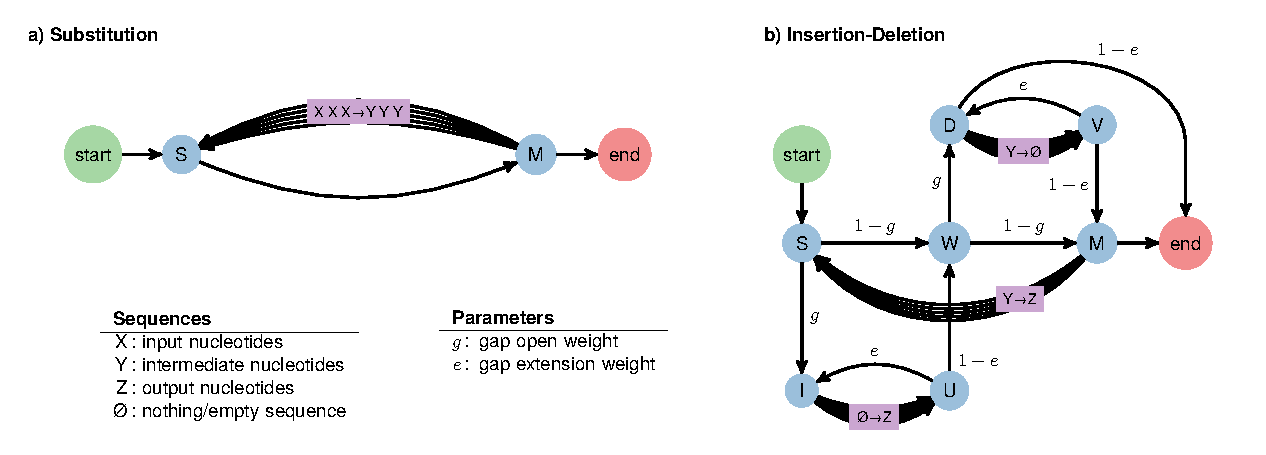
\includegraphics[width=\textwidth]{fig-evolution-fst.pdf}
\par
\caption{The Evolution FST is assembled by composing a substitution FST and an indel FST.
Each node represents a state in an FST while arcs display possible transitions between states (and their weights). Unlabeled arcs have weights of 1.
(a) The substitution FST encodes a $61 \times 61 $ codon substitution model with 3721 arcs from M to S. These arcs consume three nucleotides from the input tape and emit three nucleotides to the output tape. The weight of each arc is a conditional probability derived from a codon substitution model.
(b) The indel FST allows for insertions (I to U) and deletions (D to V). Insertion arcs are weighted according to the codon model's stationary distribution of nucleotides, and deletion arcs have a weight of 1. On top of the indel FST, we add a base-calling-error FST (Supplemental Materials Figure 5) to model sequencing errors. Contiguous insertions and deletions are always arranged for insertions to precede deletions to limit equivalent alignments.}
\label{fig:evolution-fst}
\end{figure}

Codon substitution models are uncommon in sequence aligners, despite their extensive use in phylogenetics.
COATi implements the Muse and Gaut (\citeyear{muse_gaut_1994}) codon model (codon-triplet-mg) and the Empirical Codon Model \citembe{kosiol_ECM_2007} (codon-triplet-ecm).
It also lets the user provide a codon substitution matrix.
The default FST model (codon-triplet-mg) does not allow early stop codons in the ancestor sequence; although, it does support mutations to (early) stop codons under the assumption that these are artifacts common in low-quality data.

To reduce the runtime complexity of COATi, we have also developed an approximation of the Evolution FST that can be implemented with standard dynamic programming techniques. This approximation uses a marginal substitution model where the output nucleotides are independent of one another and only depend on the input codon and position. This produces a $\left(61 \times 3 \right) \times 4$ substitution model and eliminates the need to track dependencies between output nucleotides.

A marginal substitution model is calculated from a standard substitution model by calculating the marginal probabilities that each ancestral codon produces specific descendant nucleotides at each reading frame position.
%
Specifically, let
$P_\text{cod}\left(Y_0 \cdot Y_1 \cdot Y_2 \middle| X_0 \cdot X_1 \cdot X_2\right)$ represent transition probabilities from a standard codon model, and
%
\[
P_\text{mar}\left(Y_p = y \middle| X_0 \cdot X_1 \cdot X_2\right) =
\sum_{Y_0 \cdot Y_1 \cdot Y_2} I(Y_p = y) P_\text{cod}\left(Y_0 \cdot Y_1 \cdot Y_2 \middle| X_0 \cdot X_1 \cdot X_2\right)
\]
%
represent the marginal transition probabilities, where
$p \in \{0, 1, 2\}$ is the position of the descendant nucleotide relative to the ancestral reading frame and $I$ is an indicator function defined
%
$I(e) = \{ 1 \text{ if $e$ is true and } 0 \text{ otherwise}\}$.
%
COATi contains marginal models for both Muse and Gaut (\citeyear{muse_gaut_1994}) or the Empirical Codon Model, resulting in the marginal models codon-marginal-mg (default model) and codon-marginal-ecm.
These models emphasize the position in a codon where the substitution occurs, help restrict the effects of low-quality data in the descendant sequence, and allow more than one substitution per codon.
In combination with the indel model, alignment using the marginal model is implemented using dynamic programming.


\section*{Results and Discussion}
Using 16000 human genes and their gorilla homologous pairs from the ENSEMBL
database \parencite{ensembl_hubbard_2002}, we simulated a data set of pairwise
alignments with empirical gap patterns.
We used the data set to evaluate the accuracy of popular cutting edge aligners
Clustal$\Omega$ v1.2.4 \parencite{clustal_omega_sievers_2011},
MACSE v2.06 \parencite{ranwez_macse_2011}, MAFFT v7.407
\parencite{mafft_katoh_2002}, and PRANK v.170427 \parencite{prank_loytynoja_2014}
together with COATi.

After downloading, we removed 2232 sequences longer than 6000 nucleotides, identified 8369 sequence pairs that contained gaps identified by at least one aligner, and 5399 ungapped sequence pairs.
We then randomly introduced gap patterns extracted from all five methods into the ungapped sequence pairs to generate the benchmark alignments.
Alignment accuracy was measured using the distance metric $d_{seq}$
\parencite{metrics_blackburne_whelan_2011} between simulated and inferred
alignments.
In addition, accuracy of positive and negative selection was calculated
using the $F_1$ score by estimating $k_s$ and $k_a$ statistics
\parencite{ka_ks_li_1993}.

% Software comparison table
\begin{table}[!ht]
\centering
% \begin{table}[h!]
% \begin{adjustbox}{width=\columnwidth,center}
\definecolor{bestcolor}{RGB}{230,230,230}

\begingroup\centering
\begin{tabular}{r|ccccc}
      & \textbf{COATi} & \textbf{MAFFT} & \textbf{PRANK\footnotesize{*}} & \textbf{MACSE} & \textbf{Clustal$\Omega$}\\
\hline
Method    & Trip-MG & DNA & Codon & DNA+AA & AA\\[2pt]
%\hline
Avg alignment error ($d_{seq}$) & \cellcolor{bestcolor}0.00214 & 0.01392 & 0.02001 & 0.01351 & 0.02691\\
Perfect alignments & \cellcolor{bestcolor}5722 & 5408 & 4706 & 2860 & 2937\\
Best alignments & \cellcolor{bestcolor}5152 & 4833 & 4748 & 3754 & 2595\\
Imperfect alignments & \cellcolor{bestcolor}1066 & 1380 & 2082 & 3928 & 3851\\
% \hline
F1 score of positive selection & \cellcolor{bestcolor}98.2\pct & 86.1\pct & 88.4\pct & 81.2\pct & 71.0\pct \\
F1 score of negative selection & \cellcolor{bestcolor}99.8\pct & 98.6\pct & 98.8\pct & 98.3\pct & 97.0\pct
\end{tabular}
\par\endgroup
% \end{adjustbox}
% \end{table}


 \caption{COATi generates better alignments than other alignment algorithms. Results of COATi, PRANK, MAFFT, Clustal$\Omega$, and MACSE aligning 5399 empirically simulated sequence pairs. Perfect alignments have $d_{seq}=0$, best alignments have the lowest $d_{seq}$, and imperfect alignments have $d_{seq}>0$ when at least one aligner found a perfect alignment.}
 \label{table:comp}
\end{table}

COATi was significantly more accurate (lower $d_{seq}$) at inferring simulated alignments compared to other methods; all p-values were less than $2.2 \cdot 10^{-16}$ according to the one-tailed Wilcoxon signed rank test.
In addition, COATi produced more perfect alignments, less imperfect alignments, and more accurately retrieved events of positive selection (Table \ref{table:comp}).
It obtained better results compared to a wide variety of alignment strategies.
Clustal$\Omega$, performing a common approach of aligning via amino acid translations, obtained the highest average alignment error and had difficulties retrieving positive selection.
MACSE, which allows frameshifts, is also based on an amino acid model and obtained similar results to the DNA-based MAFFT.
PRANK, using a codon model, had a similar average alignment error to MACSE and MAFFT but had issues recovering the simulated alignments.

Despite human and gorilla sequences having a relatively short evolutionary distance, COATi showed a biologically significant improvement over other methods, with an average alignment error nine-fold smaller than the next best method.
COATi is an FST-based application that can calculate the optimal alignment
between a pair of sequences in the presence of artifacts using a statistical
model.
It will allow researchers to analyze more data with higher accuracy and
facilitate the study of important biological processes that shape genomic data.


\section*{Availability}
The source code for COATi, along with documentation, is
freely available on GitHub: \url{https://github.com/CartwrightLab/coati} and is
implemented in C++.
Code to replicate the analysis can be found on GitHub: \url{https://github.com/jgarciamesa/coati-testing}.

% \section*{Supplementary information}

\section*{Acknowledgments}

This research was funded by NSF award DBI-1929850.\\

\noindent \textit{Conflict of interest:} none declared.

% \section{References}
\bibliographystyle{mbe}%
\setlength{\bibhang}{0pt}
\bibliography{alignpair_letter.bib}

\nolinenumbers

\end{document}
